\documentclass[conference]{IEEEtran}
\IEEEoverridecommandlockouts

\usepackage{cite}
\usepackage{amsmath,amssymb,amsfonts}
\usepackage{graphicx}
\usepackage{textcomp}
\usepackage{xcolor}
\usepackage{booktabs}
\usepackage{array}
\usepackage[hyphens]{url}
\usepackage[hidelinks]{hyperref}

\def\BibTeX{{\rm B\kern-.05em{\sc i\kern-.025em b}\kern-.08em
    T\kern-.1667em\lower.7ex\hbox{E}\kern-.125emX}}

\begin{document}

\title{A Machine Learning Model for Real-Time Personalized Feedback in Introductory Programming}

\author{
    \IEEEauthorblockN{Alimzhan Koshikov}
    \IEEEauthorblockA{
        \textit{School of Software Engineering}\\
        Astana IT University\\
        Astana, Kazakhstan\\
        225148@astanait.edu.kz\\
        \href{https://orcid.org/0009-0003-3234-6487}{ORCID: 0009-0003-3234-6487}
    }
    \and
    \IEEEauthorblockN{Shyryn Tutkyshbayeva}
    \IEEEauthorblockA{
        \textit{School of Software Engineering}\\
        Astana IT University\\
        Astana, Kazakhstan\\
        sh.tutkyshbayeva@astanait.edu.kz\\
        \href{https://orcid.org/0000-0002-1419-2571}{ORCID: 0000-0002-1419-2571}
    }
}

\maketitle

\begin{abstract}
Virtual mentors for novice programmers need a reliable decision layer before they generate feedback. This paper studies that layer as a supervised machine learning problem for real-time personalized support in introductory programming. The model is connected to SocratesAI, a web-based prototype where a student submits code, the backend requests a feedback-state prediction, a bounded hint is generated, and the prediction is stored in interaction logs for later analysis. A public dataset of Python Codeforces submissions was filtered to beginner-level problems and mapped from judge outcomes into five feedback states: accepted, semantic debugging, execution safety, efficiency review, and syntax repair. The experimental frame contains 178414 submissions from 872 problems and is evaluated with a problem-level holdout. A source-code model based on hashed character n-grams achieved macro $F_1=0.426$, compared with $0.085$ for the majority baseline. A model that also uses run results achieved macro $F_1=0.814$. The results show that source code is useful for early estimates, but run results are needed for more reliable real-time feedback.
\end{abstract}

\begin{IEEEkeywords}
virtual mentor, programming education, machine learning, automated feedback, Codeforces, SocratesAI
\end{IEEEkeywords}

\section{Introduction}

Introductory programming is often a challenging subject because beginners must learn many things during the course, including syntax, algorithmic thinking, and debugging skills. During the course, students submit different codes within a coding task which causes different types of errors such as syntax error, time limit failure, wrong answer, etc. Frequently, these error traces are not sufficient to understand a problem, so it is important to provide precise and helpful feedback for each type of error. For example, syntax error needs a local repair hint, a time limit error needs a question about time complexity, and a wrong answer/output needs hint related to test cases or edge cases.

Many recent applications for programming education use large language models (LLMs) to write explanation or hints \cite{Denny2024,Ahamed2025,CodeAid2024,Iris2024}, and this is quite useful. However, it is also important to consider one important question: before the virtual assistant writes a feedback message, what kind of feedback is really appropriate for the student's current situation when he gets stuck on some task? If this decision is wrong, the generated text can eventually mislead a student and react to the wrong signal.  

So, this paper is focused on the decision layer of a virtual programming mentor. Instead of focusing on a complete tutoring system, the study examine whether the machine learning model can predict the appropriate feedback state from a student’s code and, if available, run the results. During the study, we implemented virtual assistant called SocratesAI which is a Spring Boot backend application combined with Python ML service. It was used as an implementation context: the Spring Boot backend calls a Python ML service, receives a predicted feedback state and confidence score, uses that state to guide feedback generation, and stores the prediction in \texttt{interaction\_logs}.

The paper addresses the following research questions:
\begin{itemize}
    \item \textbf{RQ1.} Can a learned feedback-state model generalize to submissions from beginner-level problems that were not used during training?
    \item \textbf{RQ2.} How much does prediction quality improve when source code is combined with run results such as passed tests, time, and memory?
    \item \textbf{RQ3.} Which feedback states remain unreliable, and how should SocratesAI handle low-confidence predictions?
\end{itemize}

The novelty of this work is not only that a classifier is trained on programming submissions. The paper studies this classifier as a feedback-state decision layer before hint generation. More specifically, it gives an operational mapping from judge outcomes to mentor states, evaluates the model with a problem-level holdout on 178,414 real submissions, compares source-only evidence with code-and-run evidence, and shows the integration path into SocratesAI through the Spring Boot backend, Python ML service, and \texttt{interaction\_logs}.


\section{Related Work}

Automated assessment and feedback tools have been used in programming education for many years. Surveys by Messer et al. \cite{Messer2024} and Kumar et al. \cite{Kumar2025} show that these systems are useful when working with many students, but they usually focus on correctness, test results, or syntax-level feedback. However, a virtual mentor needs a more explicit intermediate representation. Before generating the final response, it should first understand what kind of help is appropriate for the student.

This problem became more important with the growth of LLM-based teaching assistants. Denny et al. discuss the key properties that AI teaching assistants should have in programming education, such as reliability and alignment with learning goals \cite{Denny2024}. CodeAid evaluates the use of an LLM-based programming assistant in a real classroom and shows how such tools can balance the needs of both students and educators \cite{CodeAid2024}. Iris explores an AI-driven virtual tutor for computer science education \cite{Iris2024}, while Ahmed et al. study whether AI-augmented feedback can be feasible in CS1 courses \cite{Ahamed2025}. Overall, these works show that feedback quality is not only about generating good natural language. The timing of feedback, the type of intervention, and the amount of help revealed to the student are also important.


Other studies focus on student behaviour around AI help. Sheese et al. show that students may develop different help-seeking patterns when they use LLM-powered programming assistants \cite{Sheese2024}. Marwan et al. show that immediate adaptive feedback can support programming learning when feedback is tied to the learner's current state \cite{Marwan2022}. These findings motivate the present work: before SocratesAI phrases a hint, it should estimate the feedback need from observable evidence.

\section{Method}

\subsection{Feedback-State Formulation}

Let
\[
D=\{(x_i,y_i,g_i)\}_{i=1}^{n}
\]
be a dataset of programming submissions. Here $x_i$ is the observable submission information, $y_i$ is the feedback state, and $g_i$ is the problem identifier. The feature vector is
\[
x_i=(c_i,m_i,e_i),
\]
where $c_i$ is source code, $m_i$ contains problem and static-code metadata, and $e_i$ contains optional run-result signals.

The feedback state is a compact class describing the type of intervention needed by the mentor. In this paper,
\[
\begin{aligned}
Y=\{&\text{accepted},\text{semantic debug},\text{execution safety},\\
&\text{efficiency review},\text{syntax repair}\}.
\end{aligned}
\]
The states are derived from official judge outcomes. The exact mapping used before filtering and training is shown in Table~\ref{tab:outcomemap}. For example, a wrong answer is treated as a semantic-debug need, a time limit failure as efficiency review, a runtime or memory failure as execution safety, and a compilation error as syntax repair. This mapping is not a teacher-written hint. It is an operational target for the decision layer; the mentoring interpretation is summarized in Table~\ref{tab:taxonomy}.

\begin{table}[t]
\caption{Mapping from judge outcomes to feedback states}
\label{tab:outcomemap}
\centering
\footnotesize
\setlength{\tabcolsep}{4pt}
\renewcommand{\arraystretch}{1.12}
\begin{tabular}{>{\ttfamily\raggedright\arraybackslash}p{4.1cm}p{2.25cm}}
\toprule
\textbf{Codeforces outcome} & \textbf{Feedback state} \\
\midrule
OK & Accepted \\
WRONG\_ANSWER, PARTIAL, FAILED, REJECTED, CHALLENGED, SKIPPED & Semantic debug \\
RUNTIME\_ERROR, MEMORY\_LIMIT\_EXCEEDED, CRASHED & Execution safety \\
TIME\_LIMIT\_EXCEEDED, IDLENESS\_LIMIT\_EXCEEDED & Efficiency review \\
COMPILATION\_ERROR & Syntax repair \\
\bottomrule
\end{tabular}
\end{table}

\begin{table}[t]
\caption{Feedback-state taxonomy used for model training}
\label{tab:taxonomy}
\centering
\renewcommand{\arraystretch}{1.12}
\begin{tabular}{p{2.5cm}p{4.7cm}}
\toprule
\textbf{Feedback state} & \textbf{Typical mentoring decision} \\
\midrule
Accepted & Do not interrupt with corrective feedback. \\
Semantic debug & Ask about logic, boundary cases, or expected versus actual output. \\
Execution safety & Focus on unsafe operations, indexing, recursion depth, or memory use. \\
Efficiency review & Guide the student toward complexity and repeated work. \\
Syntax repair & Localize language-form errors before conceptual feedback. \\
\bottomrule
\end{tabular}
\end{table}

A classifier estimates
\[
\hat{y}_i=f(\phi(x_i)),
\]
where $\phi(\cdot)$ is a feature representation. For the linear models used here, each class has a score
\[
s_k(x_i)=w_k^\top \phi(x_i)+b_k.
\]
The parameters are fitted by regularized logarithmic loss:
\[
\min_{W,b}-\sum_{i=1}^{n}\log P(y_i\mid \phi(x_i);W,b)
+\lambda\sum_{k}\|w_k\|_2^2.
\]
Problems are separated between training and testing:
\[
G_{\mathrm{train}}\cap G_{\mathrm{test}}=\varnothing.
\]
This split is stricter than a random row split because it tests whether the model works on new tasks, not only on new submissions to already seen tasks.

\subsection{Dataset and Features}

The empirical source is a local copy of the Codeforces Python submissions dataset \cite{MatrixStudio2026}. It was selected because it fixes the programming language family, contains accepted and failed submissions, provides official judge outcomes, and includes run-result fields such as passed tests, time, and memory.

The original dataset contains 690396 Python code submissions. It was decided to filter the dataset and leave only beginner level problems with rating at most 1200 and also remove outcomes outside the taxonomy. This leaves 490357 suitable code submissions from 881 problems. In order to reduce domination of the ewo largest classes while keeping minority states, accepted and semantic-debug rows are capped at 50000 each. Ultimately, the final version of dataset contains 178414 submissions from 872 problems.

Source code from the submissions is represented by hashed character $3$--$5$-grams. This means that the code is divided into small fragments of three to five characters, which are then used as features for the model. This representation is useful for programming code because even small parts of the code can contain important information. For example, operators, indentation patterns, short expressions, and identifier shapes can still be meaningful, even when the exact variable names or tokens are different.

In addition to the code fragments, several static metrics are also extracted from each submission. These include the number of lines, source length, branches, loops, functions, imports, input calls, print calls, and exception-handling logic. These features help describe the structure and complexity of the submitted solution.

The problem context is also included in the feature set. It contains the problem rating, problem tags, and the Python variant used in the submission. In the code-and-run setting, execution-related features are added as well, including the number of passed tests, execution time in milliseconds, and memory usage in bytes.

The main classifier used in this work is Scikit-learn's \texttt{SGDClassifier} with logarithmic loss and $L_2$ regularization \cite{Pedregosa2011}. This classifier was chosen because the generated feature vectors are sparse and high-dimensional. In this case, a linear stochastic-gradient model is a practical choice because it trains quickly, can be rerun with fixed settings, and can be serialized directly into the Python service used by SocratesAI.

This model is used as a first practical step before moving to more complex neural models. At this stage, the goal is to understand how much mentoring signal can already be extracted from simple code fragments, static metrics, problem context, and execution results. Therefore, \texttt{SGDClassifier} works as a clear and efficient baseline for making feedback-state predictions from user-submitted code.

The final run used 65536 hashed code features and 60 stochastic-gradient epochs for each linear classifier. One epoch means one complete pass through the training partition. The split contains 135752 training submissions from 654 problems and 42662 test submissions from 218 problems.

\begin{table}[t]
\caption{Training cycle used for each model variant}
\label{tab:trainingcycle}
\centering
\renewcommand{\arraystretch}{1.08}
\begin{tabular}{p{1.8cm}p{5.2cm}}
\toprule
\textbf{Stage} & \textbf{Operation} \\
\midrule
Data frame & Read parquet files, filter beginner-level problems, map judge outcomes to feedback states. \\
Split & Hold out complete problems, not only individual rows. \\
Features & Build hashed code n-grams and add selected context, metric, and run-result fields. \\
Epoch loop & For epochs $e=1,\ldots,60$, make one pass over the 135752 training submissions and update the linear classifier. \\
Evaluation & Test once on 42662 submissions from unseen problems and compute aggregate, per-class, and confusion-matrix results. \\
Artifact & Save the fitted pipeline for the Python prediction service. \\
\bottomrule
\end{tabular}
\end{table}

\begin{figure}[t]
\centering
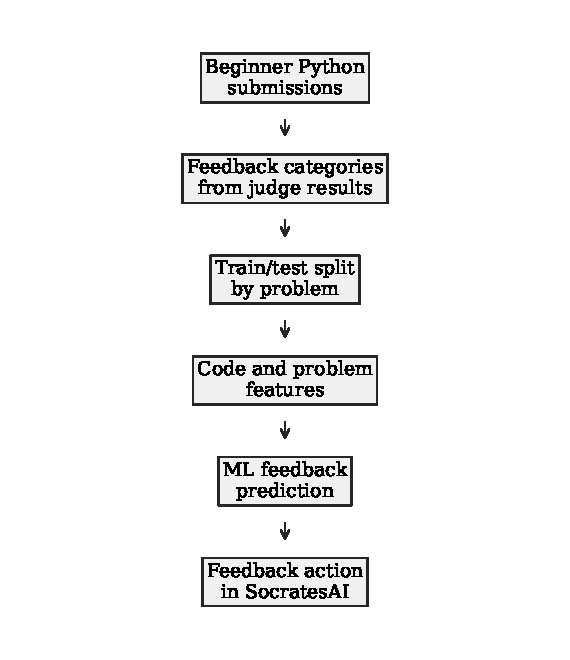
\includegraphics[width=0.78\linewidth]{figures/Figure1_ml_pipeline.pdf}
\caption{Pipeline from beginner programming submissions to a feedback-state model used by SocratesAI. Test problems are kept separate from training problems.}
\label{fig:pipeline}
\end{figure}

\section{Experimental Results}

Five models are compared: a majority baseline, a context-metrics model, a source-code model, a source-context model, and a code-and-run model. The reported metrics are accuracy, balanced accuracy, macro $F_1$, and weighted $F_1$. Macro $F_1$ is the main metric because the mentor should not be evaluated only on the largest classes.

Table~\ref{tab:results} shows the model comparison. The majority baseline performs poorly under macro $F_1$ because it predicts only the largest class. Context and static metrics alone improve the result only modestly. Source code is more informative: the source-code model reaches macro $F_1=0.426$ and balanced accuracy $0.425$ on unseen problems. This is not reliable enough for autonomous tutoring, but it is clearly above the baseline and shows that code structure contains a real feedback signal.

\begin{table}[t]
\caption{Model performance on held-out problems}
\label{tab:results}
\centering
\renewcommand{\arraystretch}{1.1}
\begin{tabular}{lrrrr}
\toprule
\textbf{Model} & \textbf{Acc.} & \textbf{Bal. acc.} & \textbf{Macro $F_1$} & \textbf{W. $F_1$} \\
\midrule
Majority & 0.2716 & 0.2000 & 0.0854 & 0.1161 \\
Context metrics & 0.3342 & 0.3483 & 0.3102 & 0.3040 \\
Source code & 0.4051 & 0.4248 & 0.4262 & 0.4045 \\
Source + context & 0.4039 & 0.4240 & 0.4121 & 0.3941 \\
Code + run results & 0.7808 & 0.8207 & 0.8137 & 0.7763 \\
\bottomrule
\end{tabular}
\end{table}

The strongest result is obtained when run results are added. The code-and-run model reaches macro $F_1=0.814$ and balanced accuracy $0.821$. This does not mean the mentor should simply repeat the judge outcome. The point is narrower: if SocratesAI has test-run evidence, it should treat this evidence as a central modelling signal, not only as a final grade.

\begin{figure}[t]
\centering
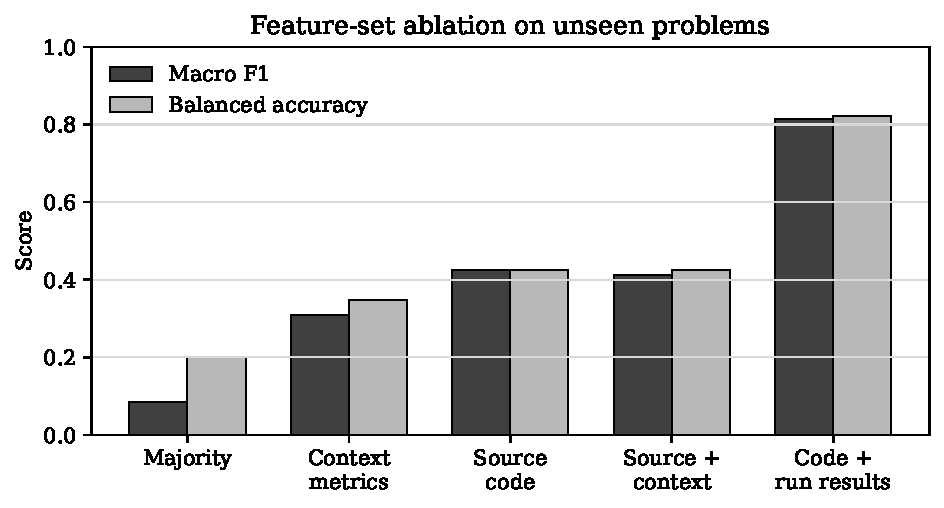
\includegraphics[width=\linewidth]{figures/Figure3_feature_set_comparison.pdf}
\caption{Feature-set ablation. Source code improves over context metrics, while run results substantially improve the decision layer.}
\label{fig:ablation}
\end{figure}

The per-class scores in Table~\ref{tab:perclass} are more useful than looking only at the overall metrics. They show how well the model works for each feedback state separately. The source-code model performs best on syntax repair and efficiency review. This is reasonable because syntax mistakes, repeated code patterns, and inefficient structures can often be noticed directly from the source code, even before the program is executed.

At the same time, the source-code model is weaker on accepted and semantic-debug states. This is also expected because two solutions may look very similar in the code, but one of them can still fail on hidden tests. In this case, source code alone does not always provide enough information to understand whether the solution is fully correct or whether it contains a logical mistake.

\begin{table}[t]
\caption{Per-class $F_1$ for two main model variants}
\label{tab:perclass}
\centering
\renewcommand{\arraystretch}{1.1}
\begin{tabular}{lrr}
\toprule
\textbf{Feedback state} & \textbf{Source code} & \textbf{Code + run} \\
\midrule
Accepted & 0.3803 & 0.9157 \\
Semantic debug & 0.4116 & 0.6099 \\
Execution safety & 0.3501 & 0.6114 \\
Efficiency review & 0.4398 & 0.9712 \\
Syntax repair & 0.5490 & 0.9602 \\
\bottomrule
\end{tabular}
\end{table}

Figure~\ref{fig:confusion} shows how the source-code model classifies different feedback states. The matrix is row-normalized, which means that each row shows how submissions from one true state were predicted by the model. The cells on the diagonal show correct predictions, while the other cells show where the model confused one state with another.

This is important for virtual mentoring because a wrong state prediction can lead to the wrong type of feedback. For example, accepted submissions are often confused with semantic-debug cases. Also, execution-safety problems are not concentrated in one predicted class, but are spread across several different states. This means that source code can give useful early signals about the possible feedback state, but it has clear limitations. It can help the system make an initial decision, but it is not always enough to distinguish a correct solution from a solution that only fails on specific tests.

\begin{figure}[t]
\centering
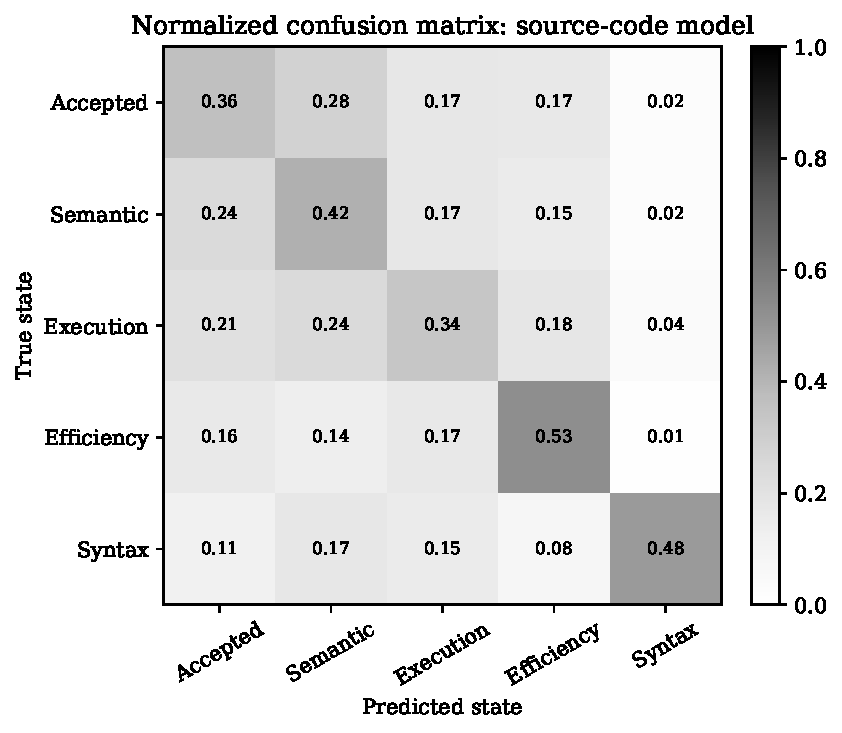
\includegraphics[width=0.93\linewidth]{figures/Figure4_confusion_matrix.pdf}
\caption{Error-classification matrix for the source-code model. Off-diagonal cells show which feedback states are confused.}
\label{fig:confusion}
\end{figure}

\section{Integration into SocratesAI}

The trained model is placed between code analysis and feedback generation layers in SocratesAI. The backend accepts and collects data including student's source code, task contexts and run results, then the backend processes request data by converting the data into a feature vector and sends to the endpoint of the Python ML service - \texttt{/predict-mentor-state}. Finally, the Python ML inference service predicts and provides full response including predicted state such as \texttt{syntax\_repair} or \texttt{efficiency\_review}, confidence scores, and a mapped feedback action.

The Spring Boot backend receives and processes the response from The Python ML Service and uses this action for feedback generation and saves the result of the prediction and confidence states in \texttt{interaction\_logs}. The Codeforces dataset is not a complete replacement for SocratesAI logs, it is a extra source for building an initial model. Additionally, logs collected in the application can significantly help in the future in conducting full classroom experiment within a programming course, as it record whether a prediction was evaluated as useful feedback by users.

The implementation has two modes: 1) source-only mode, in which the mentor can make an early estimate while the student is still editing, and should be considered as a preparatory stage to detect some basic syntax and structural errors, 2) code and-run mode, apart from basic metrics such as source code and task context, it uses test execution evidence and becomes much more reliable. It aligned with a realistic CS1 course workflow: a student writes code, runs or submits it, and receiveas a short intervention tied to the observed failure type.

The main purpose of this trained model is to select the correct pedagogical direction for student instead of just providing final hint. For example, high-confidence efficiency review prediction can consequently lead to a prompt which can help to a student with time complexity issues. A low-confidence semantic-debug prediction can lead a leading question asking the student to compare expected and actual output.  LLM is used only to phrase the selected action in natural language. The prompt for LLM is strictly limited and bounded: it should not provide a full solution, should not rewrite the student's program, and should keep the hint connected to the selected feedback state.

\begin{figure}[t]
\centering
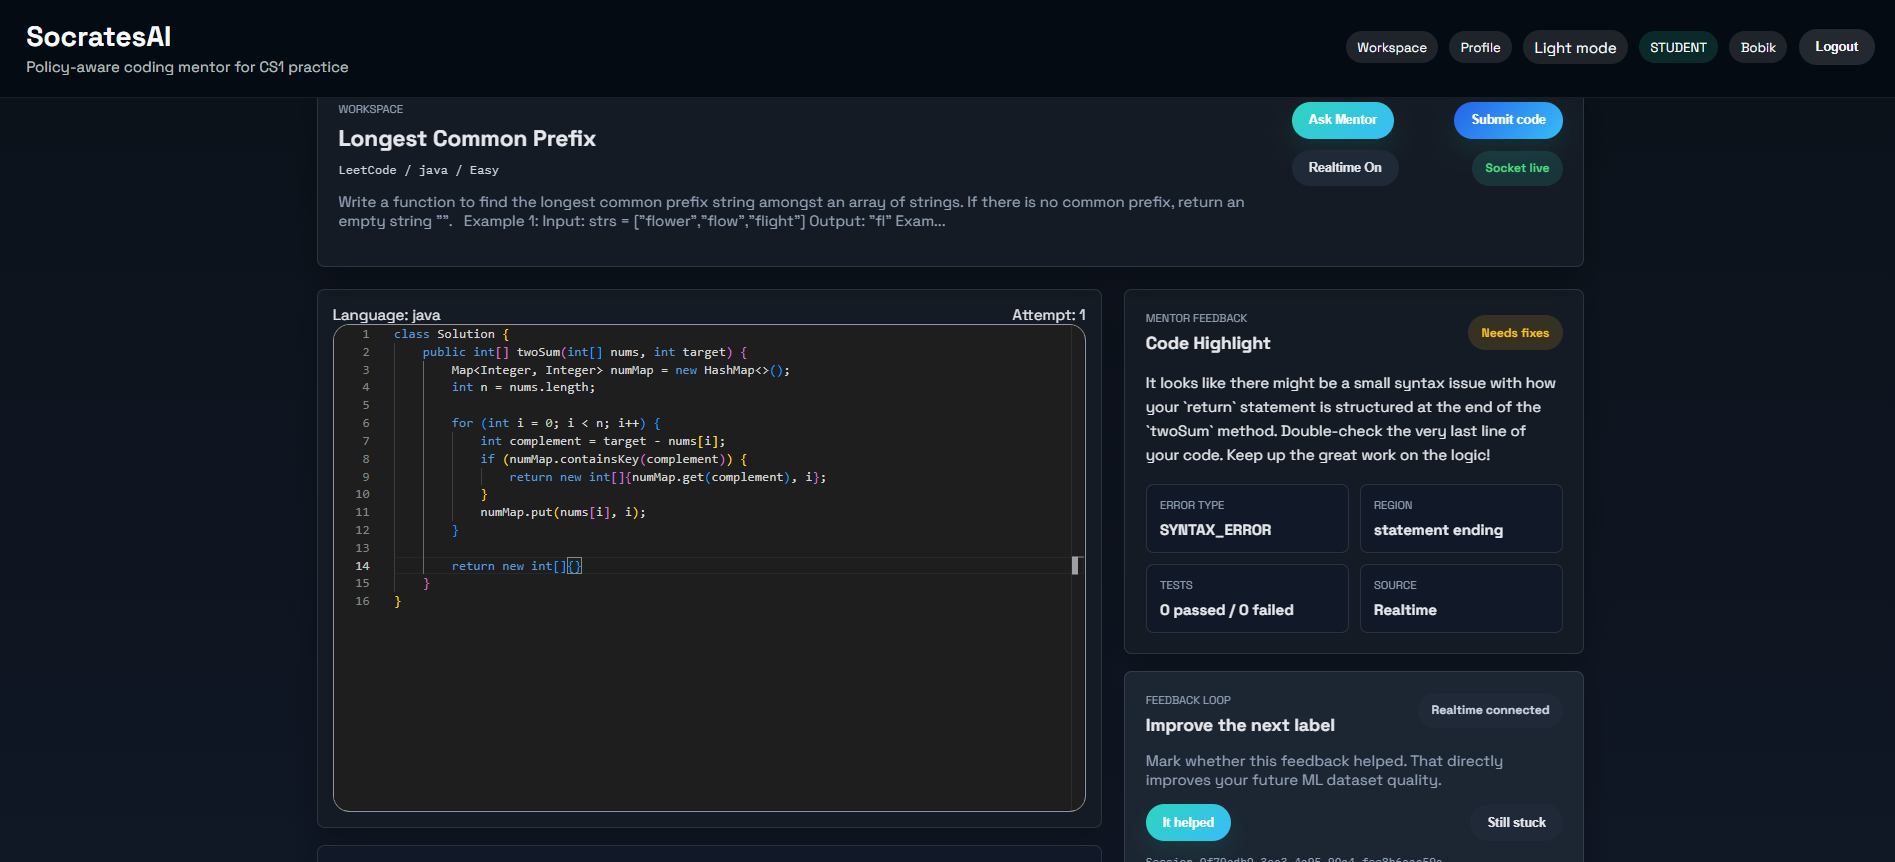
\includegraphics[width=\linewidth]{figures/interface.png}
\caption{SocratesAI interface where the model-guided feedback appears next to the student's code. The screenshot shows the deployment context; the evaluated component is the feedback-state model.}
\label{fig:interface}
\end{figure}

\section{Discussion and Limitations}

The results show that a machine learning model can learn meaningful feedback-state signals from real programming submissions, but source code alone is not enough for reliable tutoring on unseen problems. Run results change the problem substantially. This is not a weakness of the experiment; it is a design lesson for SocratesAI. A mentor that ignores passed tests, time, and memory discards evidence that helps separate failure modes.

There are also limitations.  First, Codeforces outcomes are objective judge results, not teacher-written pedagogical labels. Second, beginner-rated Codeforces problems consists only first-year programming tasks, while real classroom CS1 assignments may include style, decomposition, and explanation goals. Finally, the taxonomy is compact, the future model should distinguish more subtle error types such as off-by-one loop errors, wrong invariants, input parsing mistakes, and missing edge cases.

These limitations are acceptable for the present stage because the paper does not claim a finished educational product. It gives an empirical basement for the ML part of the mentor and shows us the next engineering step that we need to implement: keep collecting SocratesAI interaction logs, store predictions and outcomes, and validate the model on target-domain student data.

\section{Conclusion}

This paper presents virtual mentoring in introductory programming as a supervised machine learning task based on feedback states, and by using 178414 real Python submissions from beginner-level Codeforces problems, the study showed that source-code features can provide useful signals, but they are still not enough when the model is tested on unseen problems. The source-code model achieved macro $F_1=0.426$, while the code-and-run model performed much better and achieved macro $F_1=0.814$.

In conclusion, the main practical result is that a proper virtual mentor should not depend only on generating explanations or on the submitted source code, but should predict a appropriate feedback state, use code execution results when they are available, and store predictions and outcomes inside the real application in order to train the model. In SocratesAI, this approach connects the external training dataset with the implemented system: the ML service predicts the feedback state, the feedback layer turns it into a limited and relevant hint, and \texttt{interaction\_logs} become the source for future classroom evaluation.

\section*{Acknowledgment}

This work was carried out as part of the master’s degree research at Astana IT University. The authors thank the School of Software Engineering for supporting the development and evaluation of the SocratesAI prototype.

\begin{thebibliography}{00}

\bibitem{Messer2024}
M. Messer, N. C. C. Brown, M. K{\"o}lling, and M. Shi, ``Automated grading and feedback tools for programming education: A systematic review,'' \emph{ACM Transactions on Computing Education}, vol. 24, no. 1, Article 10, 2024.

\bibitem{Kumar2025}
S. S. Kumar, M. A. Lones, M. Maarek, and H. Zantout, ``Navigating the landscape of automated feedback generation techniques for programming exercises,'' \emph{ACM Transactions on Computing Education}, vol. 25, no. 4, Article 54, 2025.

\bibitem{Denny2024}
P. Denny, S. MacNeil, J. Savelka, L. Porter, and A. Luxton-Reilly, ``Desirable characteristics for AI teaching assistants in programming education,'' in \emph{Proc. ITiCSE}, 2024, pp. 408--414.

\bibitem{Ahamed2025}
U. Z. Ahmed, S. Sahai, B. Leong, and A. Karkare, ``Feasibility study of augmenting teaching assistants with AI for CS1 programming feedback,'' in \emph{Proc. ACM SIGCSE TS}, 2025, pp. 11--17.

\bibitem{CodeAid2024}
M. Kazemitabaar \emph{et al.}, ``CodeAid: Evaluating a classroom deployment of an LLM-based programming assistant that balances student and educator needs,'' in \emph{Proc. CHI}, 2024, Article 650.

\bibitem{Iris2024}
P. Bassner, E. Frankford, and S. Krusche, ``Iris: An AI-driven virtual tutor for computer science education,'' in \emph{Proc. ITiCSE}, 2024, pp. 394--400.

\bibitem{Sheese2024}
B. Sheese, M. Liffiton, J. Savelka, and P. Denny, ``Patterns of student help-seeking when using a large language model-powered programming assistant,'' in \emph{Proc. ACE}, 2024, pp. 49--57.

\bibitem{Marwan2022}
S. Marwan, B. Akram, T. Barnes, and T. W. Price, ``Adaptive immediate feedback for block-based programming: Design and evaluation,'' \emph{IEEE Transactions on Learning Technologies}, vol. 15, no. 3, pp. 406--420, 2022.

\bibitem{Pedregosa2011}
F. Pedregosa \emph{et al.}, ``Scikit-learn: Machine learning in Python,'' \emph{Journal of Machine Learning Research}, vol. 12, pp. 2825--2830, 2011.

\bibitem{MatrixStudio2026}
MatrixStudio, ``Codeforces-Python-Submissions,'' Hugging Face dataset repository, accessed May 30, 2026. [Online]. Available: \url{https://huggingface.co/datasets/MatrixStudio/Codeforces-Python-Submissions}

\end{thebibliography}

\end{document}
